\documentclass{standalone}
\usepackage{tikz}
\usepackage{ctex,siunitx}
\usepackage{tkz-euclide}
\usepackage{amsmath}
\usetikzlibrary{patterns, calc}
\usetikzlibrary {decorations.pathmorphing, decorations.pathreplacing, decorations.shapes,}
\begin{document}
\small
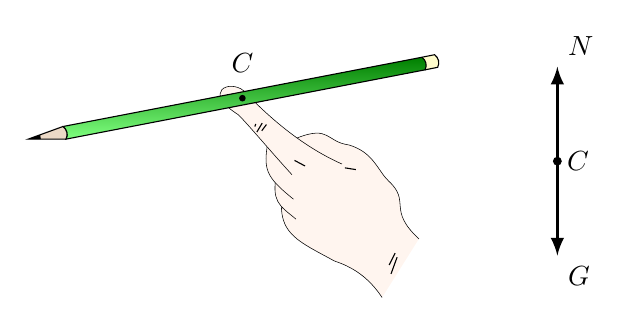
\begin{tikzpicture}[>=latex,scale=0.8]
  % \useasboundingbox (-0.1,0.1) rectangle(6,-3);
  \fill[pink!50!orange!10,draw=black,very thin]
  (2.802,-2.233)..controls(2.293,-1.763)and(2.681,-1.645)..
(2.321,-1.315)..controls(2.156,-1.164)and(2.083,-0.855)..
(1.688,-0.742)..controls(1.323,-0.690)and(1.390,-0.427)..
(0.869,-0.631)..controls(0.363,-2.103)and(0.656,-2.144)..
(1.462,-2.585)..controls(1.820,-2.701)and(2.051,-2.911)..(2.217,-3.164);
\fill[pink!50!orange!10,draw=black,very thin]
(0.543,-1.183)..controls(0.463,-1.641)and(0.569,-1.690)..(0.850,-1.919);
\fill[pink!50!orange!10,draw=black,very thin]
(1.064,-1.02)--(0.406,-0.680)..controls(0.334,-1.128)and(0.357,-1.240)..(0.811,-1.603);
\fill[pink!50!orange!10,draw=black,very thin]
( 1.581,-1.045)..controls( 1.001,-0.788)and( 0.473,-0.361)..
( 0.021, 0.118)..controls(-0.206, 0.304)and(-0.649, 0.104)..
(-0.064,-0.263)..controls( 0.112,-0.441)and( 0.404,-0.794)..( 0.786,-1.214)
;
\draw[thin](0.8275,-0.9876)--(0.9944,-1.0764);
\draw[thin](1.6277,-1.1060)--(1.8015,-1.1337);
\draw[thin](2.3308,-2.6481)--(2.4242,-2.4597);
\draw[thin](2.3593,-2.7890)--(2.4559,-2.5246);
\draw[thin](0.2120,-0.4089)--(0.1977,-0.4506);
\draw[thin](0.2297,-0.5373)--(0.3151,-0.3946);
\draw[thin](0.3079,-0.5171)--(0.3816,-0.4180);
% \draw[thin](0.2120     Y = -0.4089)--(0.1977     Y = -0.4506);(-3.4,-0.62)--

\draw[fill=yellow!20](2.85,0.65)--(3.05,0.69)[bend left=40]to(3.10,0.49)--(2.9,0.45);
  \draw[top color=green!50!black,bottom color=green!50!white]
  (-2.85,-0.45)--(2.85,0.65)[bend left=40]to(2.90,0.45)--(-2.80,-0.65)[bend right=40]to cycle;
  \draw[fill=brown!30](-2.80,-0.65)--(-3.4,-0.65)--(-2.85,-0.45)[bend left=40]to cycle;
  \fill[black](-3.21,-0.58)--(-3.4,-0.65)--(-3.2,-0.65);
  \fill(0,0)circle(1.5pt)node[above=2mm]{$C$};

  \begin{scope}[xshift=5cm,yshift=-1cm]
    \fill(0,0)circle(2pt)node[right]{$C$};
    \draw[->,very thick](0,0)--(0,1.5)node[above right]{$N$};
    \draw[->,very thick](0,0)--(0,-1.5)node[below right]{$G$};
  \end{scope}
  % \draw [-stealth](0,0) parabola (6,-3);
  % \draw[->](0,0)--++(1.2,0)node[right]{$v$};
  % \draw[->](0,0)--++(0,-0.8)node[right]{$G$};
  % \draw[->](2.4,-0.48)--++(0,-0.8)node[right]{$G$};
  % \draw[->](2.4,-0.48)--++(1.15,-0.46)node[above]{$v$};
\end{tikzpicture}
\end{document}